\section{Methodology}
The proposed methodology for the crop disease prediction system involves several key steps, starting with the collection of labeled crop image datasets that represent various diseases. The collected data will undergo preprocessing, including resizing, augmentation, and normalization, to ensure consistency and quality. Features will be extracted using deep learning models such as ResNet50, followed by the selection of an appropriate machine learning model, like a Convolutional Neural Network (CNN), for image classification. The model will be trained using a subset of the data, with hyperparameters tuned to optimize performance. Once trained, the model will be evaluated using metrics such as accuracy, precision, and recall. Optimization techniques, including fine-tuning and data augmentation, will be applied to improve the model’s performance. Finally, the trained model will be integrated into a user-friendly application that allows real-time crop disease predictions, and the system will be continuously monitored and updated based on user feedback and new data.

\subsection{Proposed Approach}
The project will utilize a deep learning-based supervised learning approach. The labeled dataset of crop images will serve as the input to train a convolutional neural network (CNN) for image classification tasks. The supervised learning approach ensures that the model learns to map input images to corresponding disease labels effectively.

\subsection{Algorithms/Models Under Consideration}
The following algorithms and models will be evaluated for their performance:
\begin{itemize}
    \item \textbf{Convolutional Neural Networks (CNNs):} The primary model for image-based classification, leveraging architectures like VGG16, ResNet, and EfficientNet.
    \item \textbf{Transfer Learning:} Pre-trained models such as MobileNet and InceptionNet will be fine-tuned on the crop disease dataset to improve accuracy and reduce training time.
    \item \textbf{Ensemble Models:} Combining predictions from multiple models to enhance reliability and performance.
\end{itemize}

\subsection{Tools, Libraries, and Frameworks}
The implementation will utilize the following tools and libraries:
\begin{itemize}
    \item \textbf{Programming Language:} Python
    \item \textbf{Libraries and Frameworks:} TensorFlow, Keras, PyTorch, OpenCV, and NumPy
    \item \textbf{Development Environment:} Jupyter Notebook, Google Colab
    \item \textbf{Visualization Tools:} Matplotlib, Seaborn, Plotly
\end{itemize}
\newpage
\subsection{Workflow}
The proposed workflow for the project is depicted in Figure~\ref{fig:methodology_workflow}, which includes the phases of data preprocessing, model training, and deployment.

\begin{figure}[h]
    \centering
    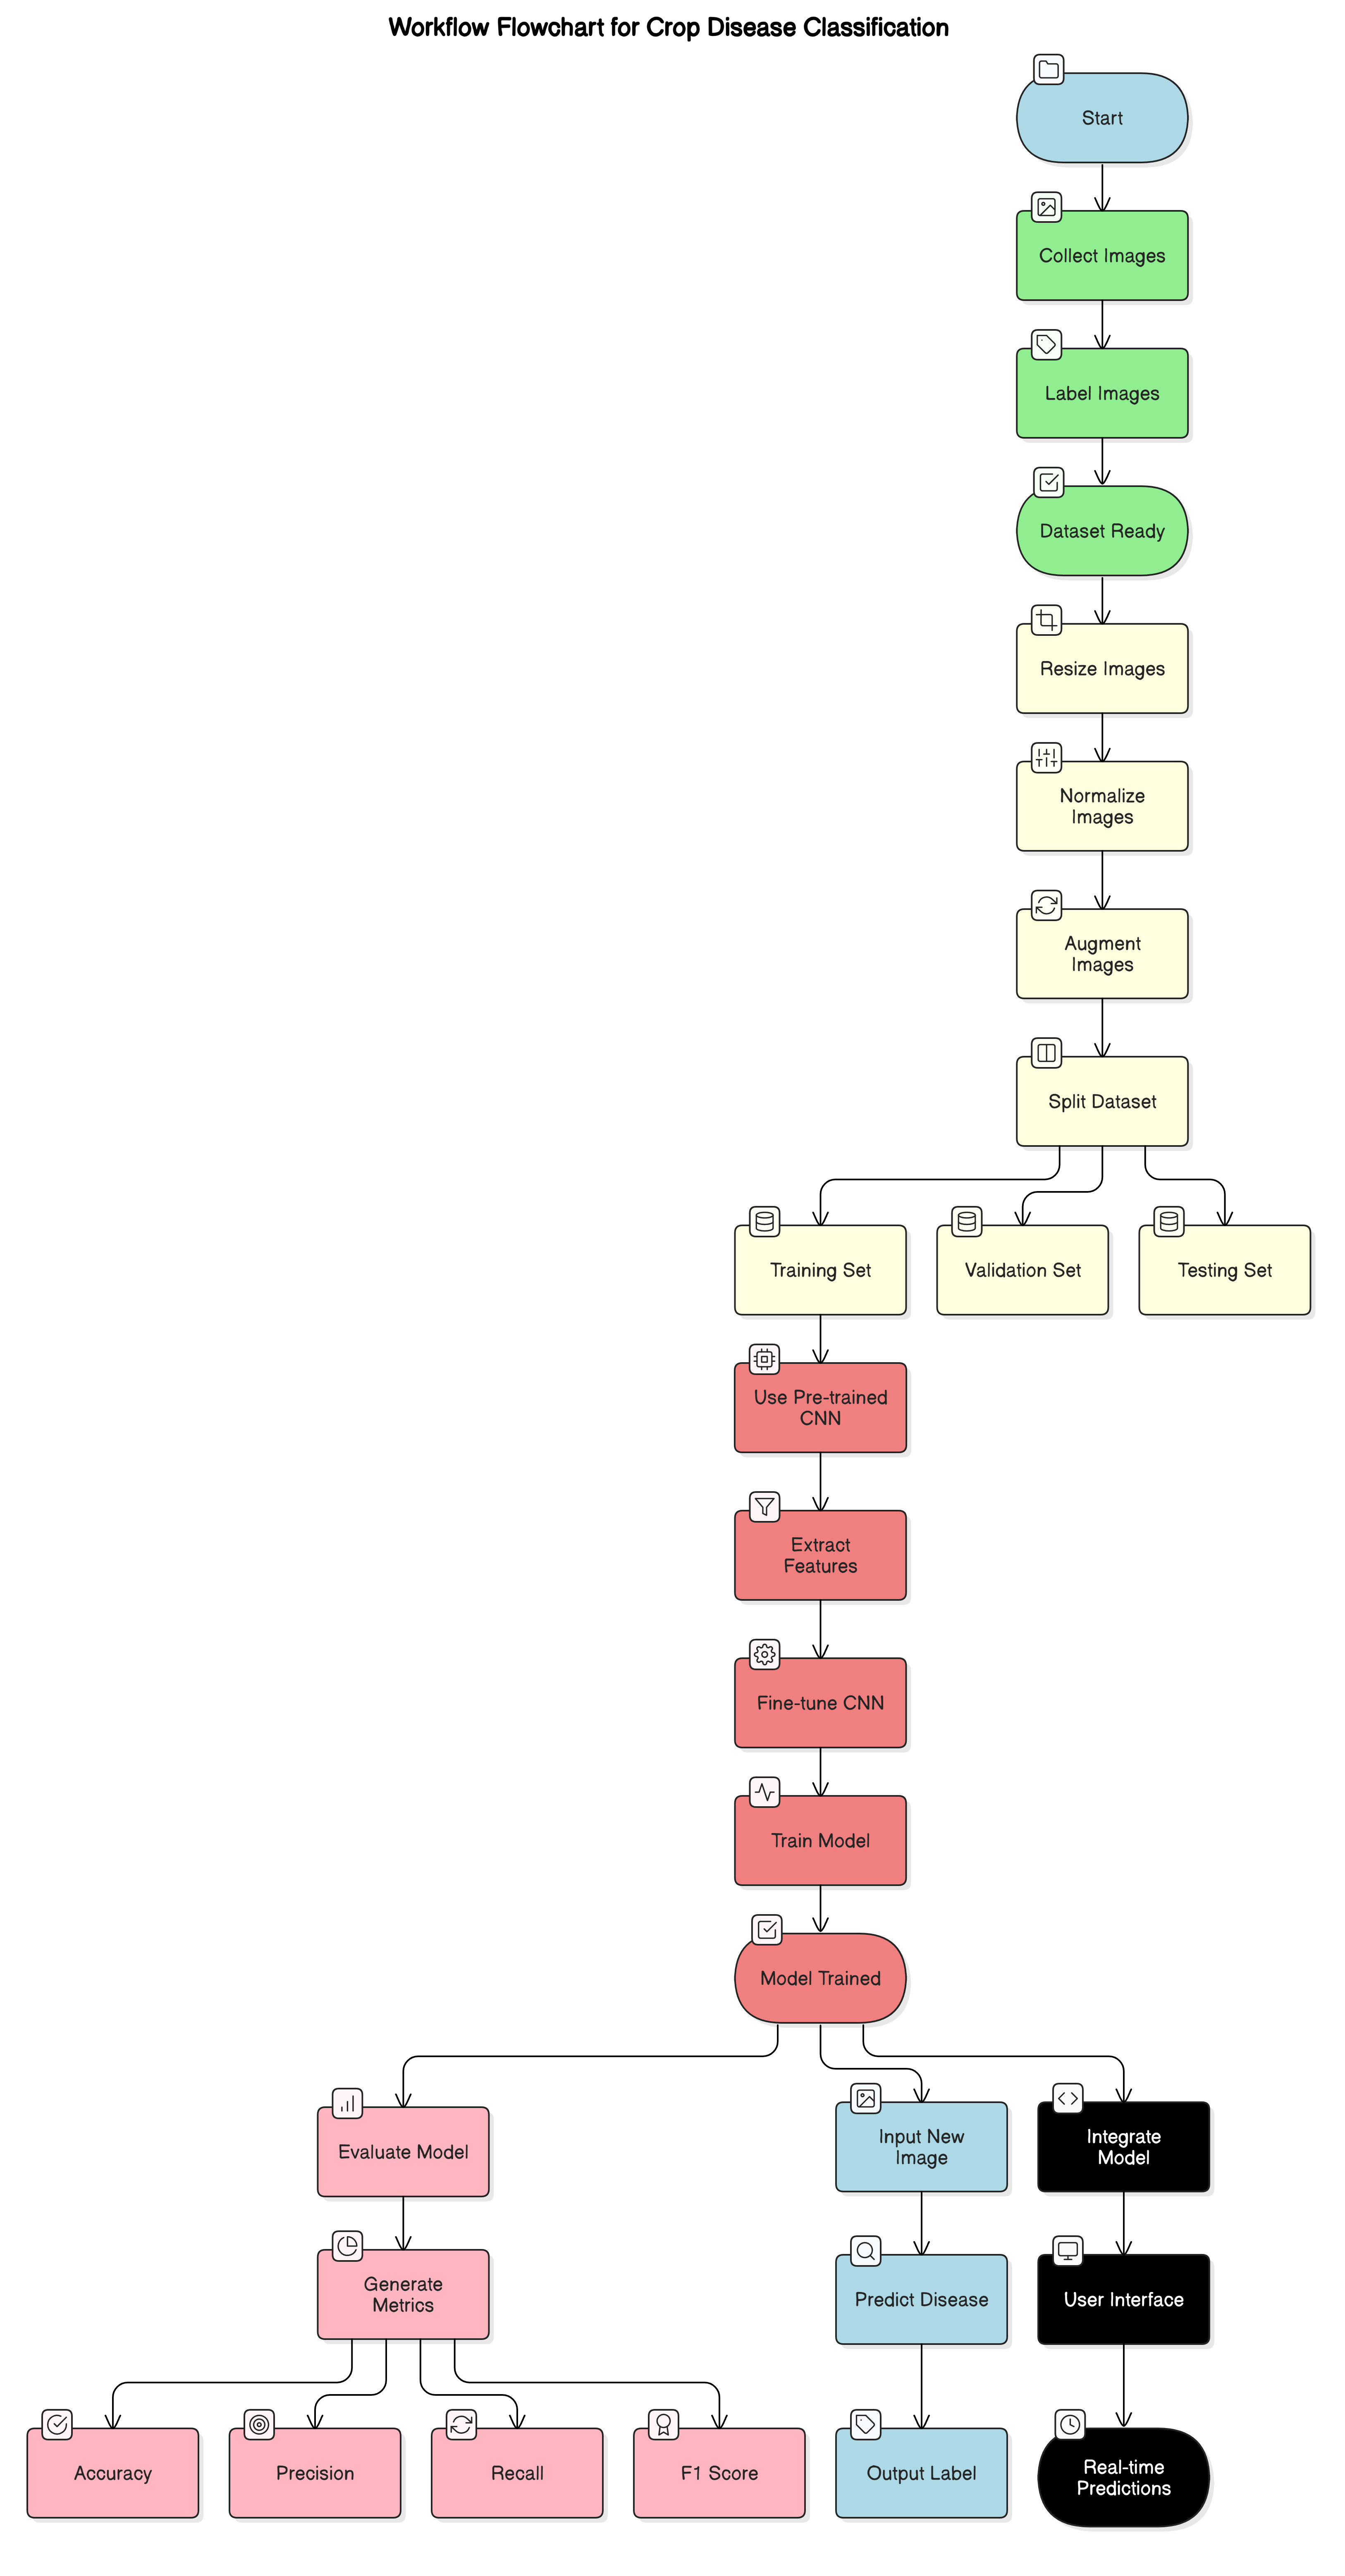
\includegraphics[width=0.6\linewidth]{Images/flow.png}
    \caption{Workflow for Crop Disease Prediction System}
    \label{fig:methodology_workflow}
\end{figure}
\newpage
\subsection{Cost-Benefit Analysis}
A sample cost-benefit analysis of the project is presented in Table~\ref{tab:cost-benefit}.
\begin{table}[h]
    \centering
    \caption{Sample Cost-Benefit Analysis of the Proposed Project}
    \label{tab:cost-benefit}
    {
    \begin{tabular}{|p{4cm}|p{4cm}|p{4cm}|p{4cm}|}
        \hline
        \textbf{Item} & \textbf{Description} & \textbf{Cost (\$)} & \textbf{Benefit (\$)} \\ \hline
        Planning & Define objectives, scope, and deliverables & 2,000 & Clear and actionable project roadmap \\ \hline
        Data Preparation & Collect and preprocess datasets & 3,500 & High-quality and usable data for modeling \\ \hline
        Model Development & Select, train, and fine-tune the model & 5,000 & Robust machine learning model for crop disease classification \\ \hline
        Testing & Evaluate and test the model & 2,000 & Reliable and accurate predictions validated \\ \hline
        Deployment & Integrate and deploy the system & 3,000 & Fully functional system ready for end-users \\ \hline
        Documentation & Prepare documentation and reports & 1,000 & Comprehensive project resources for future reference \\ \hline
        Application Development & Create a user-friendly application & 2,000 & Accessible tool for real-time disease detection \\ \hline
        \textbf{Total Costs} &  & \textbf{18,500} & - \\ \hline
        Productivity Gains & Time and resource savings for farmers & - & 25,000 \\ \hline
        Increased Revenue & Improved crop yields & - & 15,000 \\ \hline
        User Satisfaction & Enhanced user experience and feedback & - & 10,000 \\ \hline
        \textbf{Total Benefits} &  & - & \textbf{50,000} \\ \hline
        \textbf{Net Benefit} &  & \textbf{18,500} & \textbf{31,500} \\ \hline
    \end{tabular}
    }
\end{table}
